\chapter{Graphene}

\section{Graphene}

Graphene is a two dimensional honeycomb lattice of carbon atoms. Each carbon atom is $sp^2$ hybridized where one $s$ orbital and two $p$ orbitals form three planar bonds with a separation angle of 120\degree. The distance between the individual carbon atoms is 1.42 Å. Due to the flexibility of the $sp^2$ bonds in the z direction, many other structures can be formed by a sheet of graphene, such as fullerenes, carbon nanotubes, and graphite. The graphene unit cell consists of only two lattice points, and the lattice vectors can be written as the following:

\begin{align*}
  a_1 = \frac{a}{2}(3,-\sqrt{3}) \; a_2 = \frac{a}{2}(3,\sqrt{3})
\end{align*}

\section{Graphene on Ir}

As a monolayer of graphene is synthesized on top of a metal surface the underlying metal and the graphene monolayer rarely has identical lattice parameters. This causes a mismatch between the two layers and these will be rotated at an angle compared to each other. A moiré superstructure appears when this surface is examined by STM, because certain areas has carbon directly above iridium, and certain areas has carbon and iridum perfectly out of phase. Below, figure \ref{moireunitcell} shows the the graphene-iridium moiré unit cell.

\begin{figure}
  \centering
  \begin{subfigure}[b]{0.3\textwidth}
       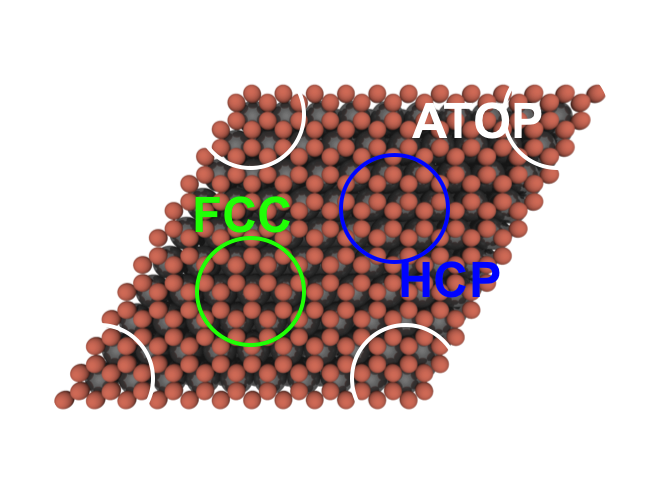
\includegraphics[width=\textwidth]{grirmoire}
       \caption{}
       \label{fig:unmarked}
   \end{subfigure}
   \begin{subfigure}[b]{0.3\textwidth}
        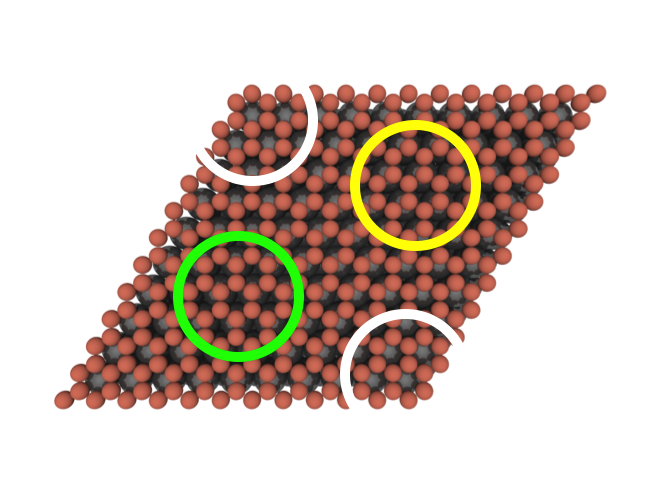
\includegraphics[width=\textwidth]{grirmoiremarked}
        \caption{}
        \label{fig:marked}
    \end{subfigure}
  \caption{Graphical interpretation of the Gr/Ir moire unit cell. \cite{Line}}
  \label{moireunitcell}
\end{figure}


\section{Hydrogenation of graphene using vibrationally excited deuterium}


\section{Hydrogenation of graphene using atomic deuterium}
